\documentclass[answers]{exam}
\usepackage{../TT2024}
\usepackage{graphicx}
\usepackage[export]{adjustbox}
\graphicspath{ {./images/} }

\title{Statistics and Data Analysis -- Sheet 4}
\author{YOUR NAME HERE :)}
\date{Trinity Term 2024}
% accurate as of 25/06/2024


\begin{document}
\maketitle
\begin{questions}

\question%1
In the model $Y_{i}=\alpha+\beta x_{i}+\epsilon_{i}, i=1, \ldots, n$, where $E\left(\epsilon_{i}\right)=0$, show that the least squares estimator of $\beta$ is \[
	\widehat{\beta}=\frac{n \sum x_{i} Y_{i}-\left(\sum x_{i}\right)\left(\sum Y_{i}\right)}{n \sum x_{i}^{2}-\left(\sum x_{i}\right)^{2}} .
\] Show that $\widehat{\beta}$ is unbiased for $\beta$. Under what additional assumptions is $\widehat{\beta}$ the maximum likelihood estimator of $\beta$?



\question%2
\begin{subparts}
\subpart Suppose $x_{1}, \ldots, x_{n}$ are known constants and that $Y_{1}, \ldots, Y_{n}$ satisfy the ``regression through the origin" model $Y_{i}=\beta x_{i}+\epsilon_{i}$, where the $\epsilon_{i}$ are independent $N\left(0, \sigma^{2}\right)$ random variables. Show that the maximum likelihood estimator of $\beta$ is $\widehat{\beta}=\sum x_{i} Y_{i} / \sum x_{i}^{2}$. What is the distribution of $\widehat{\beta}$?
\subpart Suppose we have data giving the distance, in miles, by road $\left(y_{i}\right)$ and in a straight line $\left(x_{i}\right)$ for several different journeys. Why might we prefer to consider the model above to the model $Y_{i}=\alpha+\beta x_{i}+\epsilon_{i}$?
\subpart Assuming the ``regression through the origin" model, if the straight-line distance between two locations is 12 miles, how would you use the model to predict the expected distance by road? How could we find a $95 \%$ confidence interval for this expected distance?
\end{subparts}



\question%3
\begin{subparts}
\subpart Suppose $Y_{1}, \ldots, Y_{n}$ satisfy \begin{equation}
	Y_{i}=a+b\left(x_{i}-\bar{x}\right)+\epsilon_{i}
\end{equation} where the $\epsilon_{i}$ are independent $N\left(0, \sigma^{2}\right)$ and the constants $x_{i}$ are not all equal. Find the maximum likelihood estimators $\widehat{a}$ and $\widehat{b}$. Show that $\widehat{a}$ and $\widehat{b}$ are unbiased for $a$ and $b$, respectively, and find their variances. Assuming $\sigma^{2}$ is known, show how the distribution of $\widehat{b}$ can be used to construct a $95 \%$ confidence interval for $b$.
\subpart The plot below (data from Davison (2003)) shows annual maximum sea levels in Venice for 1931-1981. Consider model (1) and also the second model \begin{equation}
	Y_{i}=\alpha+\beta x_{i}+\epsilon_{i} .
\end{equation} Give an interpretation in words of the estimates $\widehat{a}=119.6$ and $\widehat{b}=0.567$ for model (1), and $\widehat{\alpha}=-989.4$ and $\widehat{\beta}=0.567$ for model (2). From the point of view of interpreting the model, do you prefer model (1) or (2)?
\end{subparts}
\begin{center}
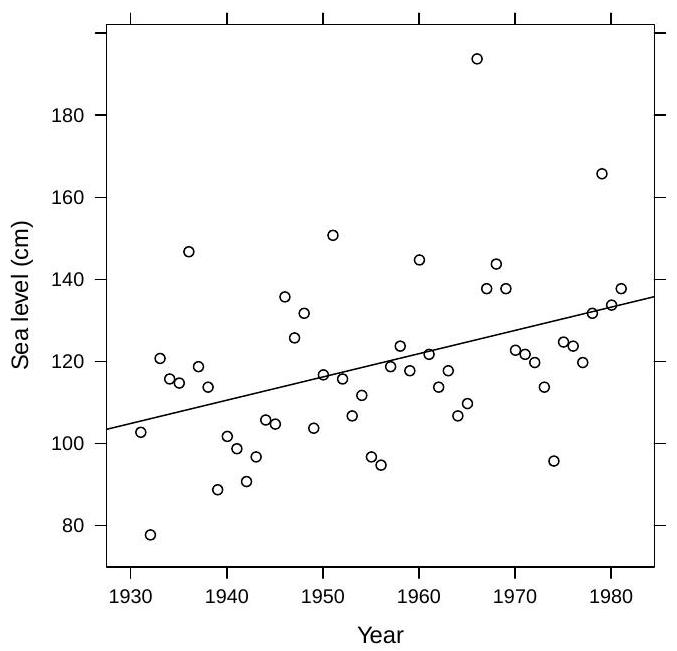
\includegraphics[max width=.45\textwidth]{sheet 4}
\end{center}



\question%4
(Using R or MATLAB)\\
$\mathrm{R}$ : work through Rdemo-2. It looks briefly at a few small datasets, check that you understand the approach taken. Most/all of the material involving residuals will be in lectures in week 3, you may want to wait until then to do some parts. For the two Olympics datasets, fit simple models and hence predict the winning times in 2012 and 2016. How do these compare to the actual winning times?\\
MATLAB: you will first need to download and read-in each dataset, see the final page of Rdemo-2.

\end{questions}

\end{document}
